%!TEX program = xelatex
\documentclass[dvipsnames, svgnames,a4paper,11pt]{article}
% ----------------------------------------------------
%   中山大学物理与天文学院本科实验报告模板
%   作者:Huanyu Shi,2019级
%   知乎:https://www.zhihu.com/people/za-ran-zhu-fu-liu-xing
%   Github:https://github.com/Huanyu-Shi/SYSU-SPA-Labreport-Template
%   Last update : 2023.4.10
% ----------------------------------------------------

% ----------------------------------------------------- 
%	加边框的命令
%	参考:https://tex.stackexchange.com/questions/531559/how-to-add-the-page-border-for-first-two-pages-in-latex
\usepackage{tikz}
\usetikzlibrary{calc}
\usepackage{eso-pic}
\AddToShipoutPictureBG{%
\begin{tikzpicture}[overlay,remember picture]
\draw[line width=0.6pt] % 边框粗细
    ($ (current page.north west) + (0.6cm,-0.6cm) $)
    rectangle
    ($ (current page.south east) + (-0.6cm,0.6cm) $); % 边框位置
\end{tikzpicture}}


\usepackage{xcolor}
\definecolor{c1}{HTML}{2752C9} % 目录颜色
\definecolor{c2}{RGB}{190,20,83} % 引用颜色

\usepackage{ctex}
\usepackage[top=28mm,bottom=28mm,left=15mm,right=15mm]{geometry}
\usepackage{hyperref} 
\hypersetup{
	colorlinks,
	linktoc = section, % 超链接位置,选项有section, page, all
	linkcolor = c1, % linkcolor 目录颜色
	citecolor = c1  % citecolor 引用颜色
}
\usepackage{amsmath,enumerate,multirow,float}
\usepackage{tabularx}
\usepackage{tabu}
\usepackage{subfig}
\usepackage{fancyhdr}
\usepackage{graphicx}
\usepackage{wrapfig}  
\usepackage{physics}
\usepackage{appendix}
\usepackage{amsfonts}

%
\usepackage{tcolorbox}
\tcbuselibrary{skins,breakable}
\newtcolorbox{tbox}[2][]{
    colframe=black!70!,
    breakable,
    enhanced,
	boxrule =0.5pt,
    title = {#2},
    fonttitle = \large\kaishu\bfseries,
	drop fuzzy shadow,
    #1
}
\newtcolorbox[auto counter,number within=section]{question}[1][]{
  top=2pt,bottom=2pt,arc=1mm,
  boxrule=0.5pt,
%   frame hidden,
  breakable,
  enhanced, %跨页后不会显示下边框
  coltitle=c1!80!gray,
  colframe=c1,
  colback=c1!3!white,
  drop fuzzy shadow,
  title={思考题~\thetcbcounter:\quad},
  fonttitle=\bfseries,
  attach title to upper,
  #1
}
\newcommand{\setLhead}[1]{%
  \lhead{{\color{gray}\kaishu #1}} % 定义新的命令,设置右边页眉的内容
}
\newcommand{\setRhead}[1]{%
  \rhead{{\color{gray}\kaishu #1}} % 定义新的命令,设置右边页眉的内容
}
% ---------------------------------------------------------------------
%	利用cleveref改变引用格式,\cref是引用命令
\usepackage{cleveref}
\crefformat{figure}{#2{\textcolor{c2}{图 #1}}#3} % 图片的引用格式
\crefformat{equation}{#2{(\textcolor{c2}{#1})}#3} % 公式的引用格式
\crefformat{table}{#2{\textcolor{c2}{表 #1}}#3} % 表格的引用格式


% ---------------------------------------------------------------------
%	页眉页脚设置
\fancypagestyle{plain}{\pagestyle{fancy}}
\pagestyle{fancy}
\setLhead{中山大学物理与天文学院基础物理实验预习报告}
%\lhead{\kaishu 中山大学物理与天文学院物理实验\uppercase\expandafter{\romannumeral3}} % 左边页眉,学院 + 课程
%\rhead{{\color{gray}\kaishu Template 实验报告模板}} % 右边页眉,实验报告标题
\setRhead{实验1\hspace{1pt}冰的熔化热测量}
\cfoot{\thepage} % 页脚,中间添加页码


% ---------------------------------------------------------------------
%	对目录、章节标题的设置
\renewcommand{\contentsname}{\centerline{\huge 目录}}
\usepackage{titlesec}
\usepackage{titletoc}
% \titleformat{章节}[形状]{格式}{标题序号}{序号与标题间距}{标题前命令}[标题后命令]
\titleformat{\section}{\centering\LARGE\songti}{}{1em}{}

% ---------------------------------------------------------------------
%   listing代码环境设置
\usepackage{listings}
\lstloadlanguages{python}
\lstdefinestyle{pythonstyle}{
backgroundcolor=\color{gray!5},
language=python,
frameround=tftt,
frame=shadowbox, 
keepspaces=true,
breaklines,
columns=spaceflexible,                   
basicstyle=\ttfamily\small, % 基本文本设置,字体为teletype,大小为scriptsize
keywordstyle=[1]\color{c1}\bfseries, 
keywordstyle=[2]\color{Red!70!black},   
stringstyle=\color{Purple},       
showstringspaces=false,
commentstyle=\ttfamily\scriptsize\color{green!40!black},%注释文本设置,字体为sf,大小为smaller
tabsize=2,
morekeywords={as},
morekeywords=[2]{np, plt, sp},
numbers=left, % 代码行数
numberstyle=\it\tiny\color{gray}, % 代码行数的数字字体设置
stepnumber=1,
rulesepcolor=\color{gray!30!white}
}




% ---------------------------------------------------------------------
%	其他设置
\def\degree{${}^{\circ}$} % 角度
\graphicspath{{./images/}} % 插入图片的相对路径
\allowdisplaybreaks[4]  %允许公式跨页 % 导入模板的相关设置
\usepackage{lipsum}
\usepackage{indentfirst}
\usepackage{pdfpages}
\usepackage{multirow}
\usepackage{subfig}
\usepackage{graphicx}
\usepackage{float} 
\usepackage{booktabs}
\renewcommand{\d}{\mathrm{d}}


%---------------------------------------------------------------------
%	正文
%---------------------------------------------------------------------
\setRhead{密里根油滴实验}%实验名称
\begin{document}


\begin{table}
	\renewcommand\arraystretch{1.7}
	\begin{tabularx}{\textwidth}{
		|X|X|X|X
		|X|X|X|X|}
	\hline
	\multicolumn{2}{|c|}{预习报告}&\multicolumn{2}{|c|}{实验记录}&\multicolumn{2}{|c|}{分析讨论}&\multicolumn{2}{|c|}{总成绩}\\
	\hline
	 & &  & &  & &  & \\
	\hline
	\end{tabularx}
\end{table}


\begin{table}
	\renewcommand\arraystretch{1.7}
	\begin{tabularx}{\textwidth}{|X|X|X|X|}
	\hline
	专业:& 物理学类 &年级:& 2023级\\
	\hline
	姓名:& 姚昊廷  & 学号:&22322091\\
	\hline
	实验时间:& 2024.11.14& 教师签名:& \\
	\hline
	\end{tabularx}
\end{table}

\begin{center}
	\LARGE 密里根油滴实验
\end{center}

\textbf{【实验报告注意事项】}
\begin{enumerate}
	\item 实验报告由三部分组成:
	\begin{enumerate}
		\item 预习报告:(提前一周)认真研读\underline{\textbf{实验讲义}},弄清实验原理;实验所需的仪器设备、用具及其使用(强烈建议到实验室预习),完成课前预习思考题;了解实验需要测量的物理量,并根据要求提前准备实验记录表格(第一循环实验已由教师提供模板,可以打印)。预习成绩低于10分(共20分)者不能做实验。
	    \item 实验记录:认真、客观记录实验条件、实验过程中的现象以及数据。实验记录请用珠笔或者钢笔书写并签名(\textcolor{red}{\textbf{用铅笔记录的被认为无效}})。\textcolor{red}{\textbf{保持原始记录,包括写错删除部分,如因误记需要修改记录,必须按规范修改。}}(不得输入电脑打印,但可扫描手记后打印扫描件);离开前请实验教师检查记录并签名。
	    \item 分析讨论:处理实验原始数据(学习仪器使用类型的实验除外),对数据的可靠性和合理性进行分析;按规范呈现数据和结果(图、表),包括数据、图表按顺序编号及其引用;分析物理现象(含回答实验思考题,写出问题思考过程,必要时按规范引用数据);最后得出结论。
	\end{enumerate}
	\textbf{实验报告就是将预习报告、实验记录、和数据处理与分析合起来,加上本页封面。}
	\item 每次完成实验后的一周内交\textbf{实验报告}(特殊情况不能超过两周)。
	\item 除实验记录外,实验报告其他部分建议双面打印。
\end{enumerate}

{\textbf{【注意事项】}
\begin{enumerate}
	\item 实验中\textbf{\textcolor{red}{禁止用手触摸极板,注意高压危险!}}
	\item 喷油器每次喷1-2次即可,\textbf{\textcolor{red}{竖直放置、防止摔碎!}}
	\item 计时时\textbf{\textcolor{red}{眼睛要平行刻度线!}}
    
\end{enumerate}}

\clearpage
\tableofcontents
\clearpage

\setcounter{section}{0}
\section{密里根油滴实验\ \textbf{预习报告}}
	
\subsection{实验目的}
\begin{enumerate}
	\item 学习用油滴实验测量电子电荷的原理。
	\item 利用静态法和动态法观测带电油滴的运动状态,测量不同带电油滴的电荷量,验证
	电荷的不连续性,测量电子电荷值e。 
	\item 了解 CCD 摄像机、光学系统的成像原理,了解显微测量方法以及视频信号处理技
	术的工程应用等。
\end{enumerate}

\subsection{仪器用具}
\begin{table}[htbp]
	\centering
	\renewcommand\arraystretch{1.6}
	% \setlength{\tabcolsep}{10mm}
	\begin{tabular}{p{0.05\textwidth}|p{0.20\textwidth}|p{0.05\textwidth}|p{0.5\textwidth}}
	\hline
	编号& 仪器用具名称 & 数量 &  主要参数(型号,测量范围,测量精度等) \\
	\hline
	1&CCD显微密立根油滴仪 &1 &ZKY-MLG-6(包括视频监视器)\\
	\hline
	2&机油及喷雾器 &1&\\
	\hline
\end{tabular}
\end{table}

\textbf{【原理概述】}\\
密里根油滴实验可测油滴带电量的分辨率小于元电荷而一般物质(如油滴)的带电量只能为元电荷的整数倍。
通过多次测量不同油滴的带电量,反推出元电荷的值。\par
单次测量的原理是受力分析,已知或计算油滴重力,浮力,阻力与电场强度。列方程可解出其带电量。\\
\textbf{【实验前思考题】}\\
\begin{question}
	为什么必须保证油滴在测量范围内做匀速运动或静止?怎样控制油滴运动?
	\tcblower
	匀速或静止时油滴处于平衡态,易于受力分析,且省去测量加速度。仔细调整电压旋钮,使得油滴在某一刻度线
	周围只做很小的布朗运动并至少持续一分钟不明显偏离刻度线。
\end{question}


\clearpage
\setLhead{中山大学物理与天文学院基础物理实验记录}
\begin{table}
	\renewcommand\arraystretch{1.7}
	\centering
	\begin{tabularx}{\textwidth}{|X|X|X|X|}
	\hline
	专业:& 物理学类 &年级:& 2023级 \\
	\hline
	姓名: &姚昊廷& 学号:&22322091  \\
	\hline
	室温:&25.0$^\circ$C&实验地点:&A524\ F4\\
	\hline
	学生签名:& & 评分: &\\
	\hline
	实验时间:& 2024.11.14& 教师签名:&\\
	\hline
	\end{tabularx}
\end{table}
\section{密里根油滴实验\ \textbf{实验记录}}
\begin{table}[H]
	\centering
	\begin{tabular}{cccc}
		\toprule
		重力加速度$g$& 油密度$\rho$ & 大气压强$p$ & 油滴下落距离$L$\\
		\midrule
		$9.789\text{m}/\text{s}^2$ & $981\text{kg}/\text{m}^3$ & $767\text{mmHg}$ & $1.6\text{mm}$ \\
		\bottomrule
	\end{tabular}
	\vspace{0.1cm}
	\begin{tabular}{cccc}
		\toprule
		极板间距$d$& 空气粘滞系数$\eta$ & 修正常数$b$ & \\
		\midrule
		$5\text{mm}$ & $1.83\times10^{-5}\text{kg}/(\text{m}\cdot\text{s})$ & $6.17\times10^{-6}\text{m}/\text{cmHg}$ &  \\
		\bottomrule
	 \end{tabular}
	 \caption{基本参数}
\end{table}


\subsection{实验内容、步骤、结果}
平衡法步骤:进行五组实验,每组选取一个(不同的)油滴,仔细调节电压旋钮使得其静止在某一刻度线周围,此时电压
即为这个油滴的平衡电压。然后测量五组其下落1.6mm的时间。便可计算出其带电量。计算公式为
$$q=\frac{18\pi}{\sqrt{2\rho_0g}}[\frac{\eta L}{t_g[1+(\frac{b}{pa})]}]^\frac{3}{2}\frac{d}{U}$$
\begin{table}[H]
	\centering
	\begin{tabular}{cccccc}
		\toprule
		测量次数& 1 & 2 & 3&4&5\\
		\midrule
		电荷量/$10^{-19}$C & 3.919&1.427 & 7.751&2.536&6.301 \\
		\bottomrule
	\end{tabular}
	 \caption{平衡法实验结果}
\end{table}
动态法步骤:进行五组实验,每组选取一个(不同的)油滴,仔细调节电压旋钮使得其静止在某一刻度线周围,此时电压
即为这个油滴的平衡电压。然后测量五组其下落1.6mm和升高电压使得油滴上升1.6mm的时间。便可计算出其带电量。计算公式为
$$q=\frac{18\pi}{\sqrt{2\rho_0g}}[\frac{\eta L}{1+(\frac{b}{pr})}]^\frac{3}{2}\frac{d}{U}(\frac{1}{t_e}+\frac{1}{t_g})(\frac{1}{t_g})^\frac{1}{2}$$
\begin{table}[H]
	\centering
	\begin{tabular}{cccccc}
		\toprule
		测量次数& 1 & 2 & 3&4&5\\
		\midrule
		电荷量/$10^{-19}$C & 10.139&13.880 & 12.781&3.796&4.092 \\
		\bottomrule
	\end{tabular}
	 \caption{动态法实验结果}
\end{table}
\subsection{实验过程中遇到的问题记录}



\clearpage
\setLhead{中山大学物理与天文学院基础物理实验分析与讨论}
\begin{table}
	\renewcommand\arraystretch{1.7}
	\begin{tabularx}{\textwidth}{|X|X|X|X|}
	\hline
	专业:& 物理学 &年级:& 2023级\\
	\hline
	姓名: &姚昊廷& 学号:&22322091 \\
	\hline
    日期:&2024.11.14 & 评分: &\\
	\hline
	\end{tabularx}
\end{table}

\section{密里根油滴实验\ \textbf{分析与讨论}}
\textbf{【分析与讨论】}(给出测量结果完成误差分析与计算)
\begin{table}[H]
	\centering
	\begin{tabular}{cccccc}
		\toprule
		测量次数& 1 & 2 & 3&4&5\\
		\midrule
		电荷量/$10^{-19}$C & 3.919&1.427 & 7.751&2.536&6.301 \\
		$n_i$&2&1&5&2&4\\
		\bottomrule
	\end{tabular}
	 \caption{平衡法电荷量及$n_i$}
\end{table}
\begin{table}[H]
	\centering
	\begin{tabular}{cccccc}
		\toprule
		测量次数& 1 & 2 & 3&4&5\\
		\midrule
		电荷量/$10^{-19}$C & 10.139&13.880 & 12.781&3.796&4.092 \\
		$n_i$&6&9&8&2&3\\
		\bottomrule
	\end{tabular}
	 \caption{动态法电荷量及$n_i$}
\end{table}
\begin{table}[H]
	\centering
	\begin{tabular}{ccc}
		\toprule
		测量方法&测量值(线性回归斜率)&相对误差\\
		\midrule
		平衡法 & 1.563&-2.45\% \\
		动态法&1.549&-3.31\%\\
		\bottomrule
	\end{tabular}
	 \caption{测量结果及误差}
\end{table}
\textbf{【实验后思考题】}
\begin{question}
	试分析本实验的主要误差来源。
	\tcblower
	\begin{enumerate}
		\item \textbf{人为计时误差}从眼睛接收到信号到仪器反应过来需要时间,导致不小的计时误差。另外仪器老化带来的系统误差也不可忽略。
		\item 两个结果的相对误差都在$10^{-2}$量级,\textbf{空气粘滞系数,油滴密度,修正常数}的参考值只有三位有效数字,其\textbf{舍入误差}也会造成不小的误差贡献。另外三者数值也与实验温度有关,直接代入$20^\circ \text{C}$的参考值,也会造成一定误差。
		\item \textbf{电压的有效数字仅有3 位},且$q\propto \frac{1}{U}$(这样写并不严谨,我们暂且不管),其舍入误差可以造
		成不小的误差贡献。另外,实验中,平衡电压较难确定,电压在约4V 的范围内随意取值并固定,在布
		朗运动的干扰下,油滴都在一分钟时间内不产生很大位移,所以电压U 可能会存在0 - 2V 的偏差。
		\item 仪器中刻度的微小偏差也不容忽视,根据计算式,$q \propto L^{\frac{3}{2}}\propto L^2$,L 每偏差1$\mu$m,则造成实验
		结果0.09\% - 0.15\% 的相对误差,这超过了2\% 的贡献。
	\end{enumerate}
\end{question}

\begin{question}
	密立根油滴实验的总结(油滴筛选、跟踪、测量……)(经验分享;体会;感想;讨论;
	建议等)。
	\tcblower
	\textbf{关于找油滴:}大部分油滴的荷质比过高,在几百伏电压下运动非常快。虽然喷一次油滴可以产生数百
	个屏幕内的油滴,但大多数不符合我们的要求。所以筛选油滴时可以打开200 - 400V 之间任意一个
	值的电压,然后喷一下油瓶,几秒钟之内荷质比过高的油滴会快速离开屏幕,然后关掉电压,不带电
	的油滴不作任何反应,带少量电荷的油滴会缓慢下降,这些油滴就是我们的目标。若没有合适的油滴,
	就再喷一下油瓶,直到找到合适的油滴为止,如此寻找油滴速度非常快。

	\textbf{关于平衡电压的误差:}室温下在调平衡电压时,布朗运动的干扰很大(可能也有气流影响),往往电
	压在约4V 的范围内,一分钟内油滴的位置都会反复上下波动,难以判断电压过高或过低。如果降低
	实验温度,或者降低气压,可以减小这项影响。
\end{question}
\clearpage
% ---------------------------------------------------------------------
%   参考文献
%   注:使用参考文献时应按照xelatex->bibtex->xelatex->xelatex顺序进行编译
\phantomsection
%\addcontentsline{toc}{section}{参考文献}
\bibliographystyle{unsrt}
\bibliography{myref}
%\begin{thebibliography}{9}
	%\bibitem{ref1} 凤飞龙,黄育红,金蔚,王公正,崔致远,“外推法计算冰的熔解热的理论依据及Matlab实现方案”,《大学物理》,第42卷,第2期
%\end{thebibliography}


\clearpage
\appendix
\appendixpage
\addappheadtotoc
%\subsection*{相图代码}
%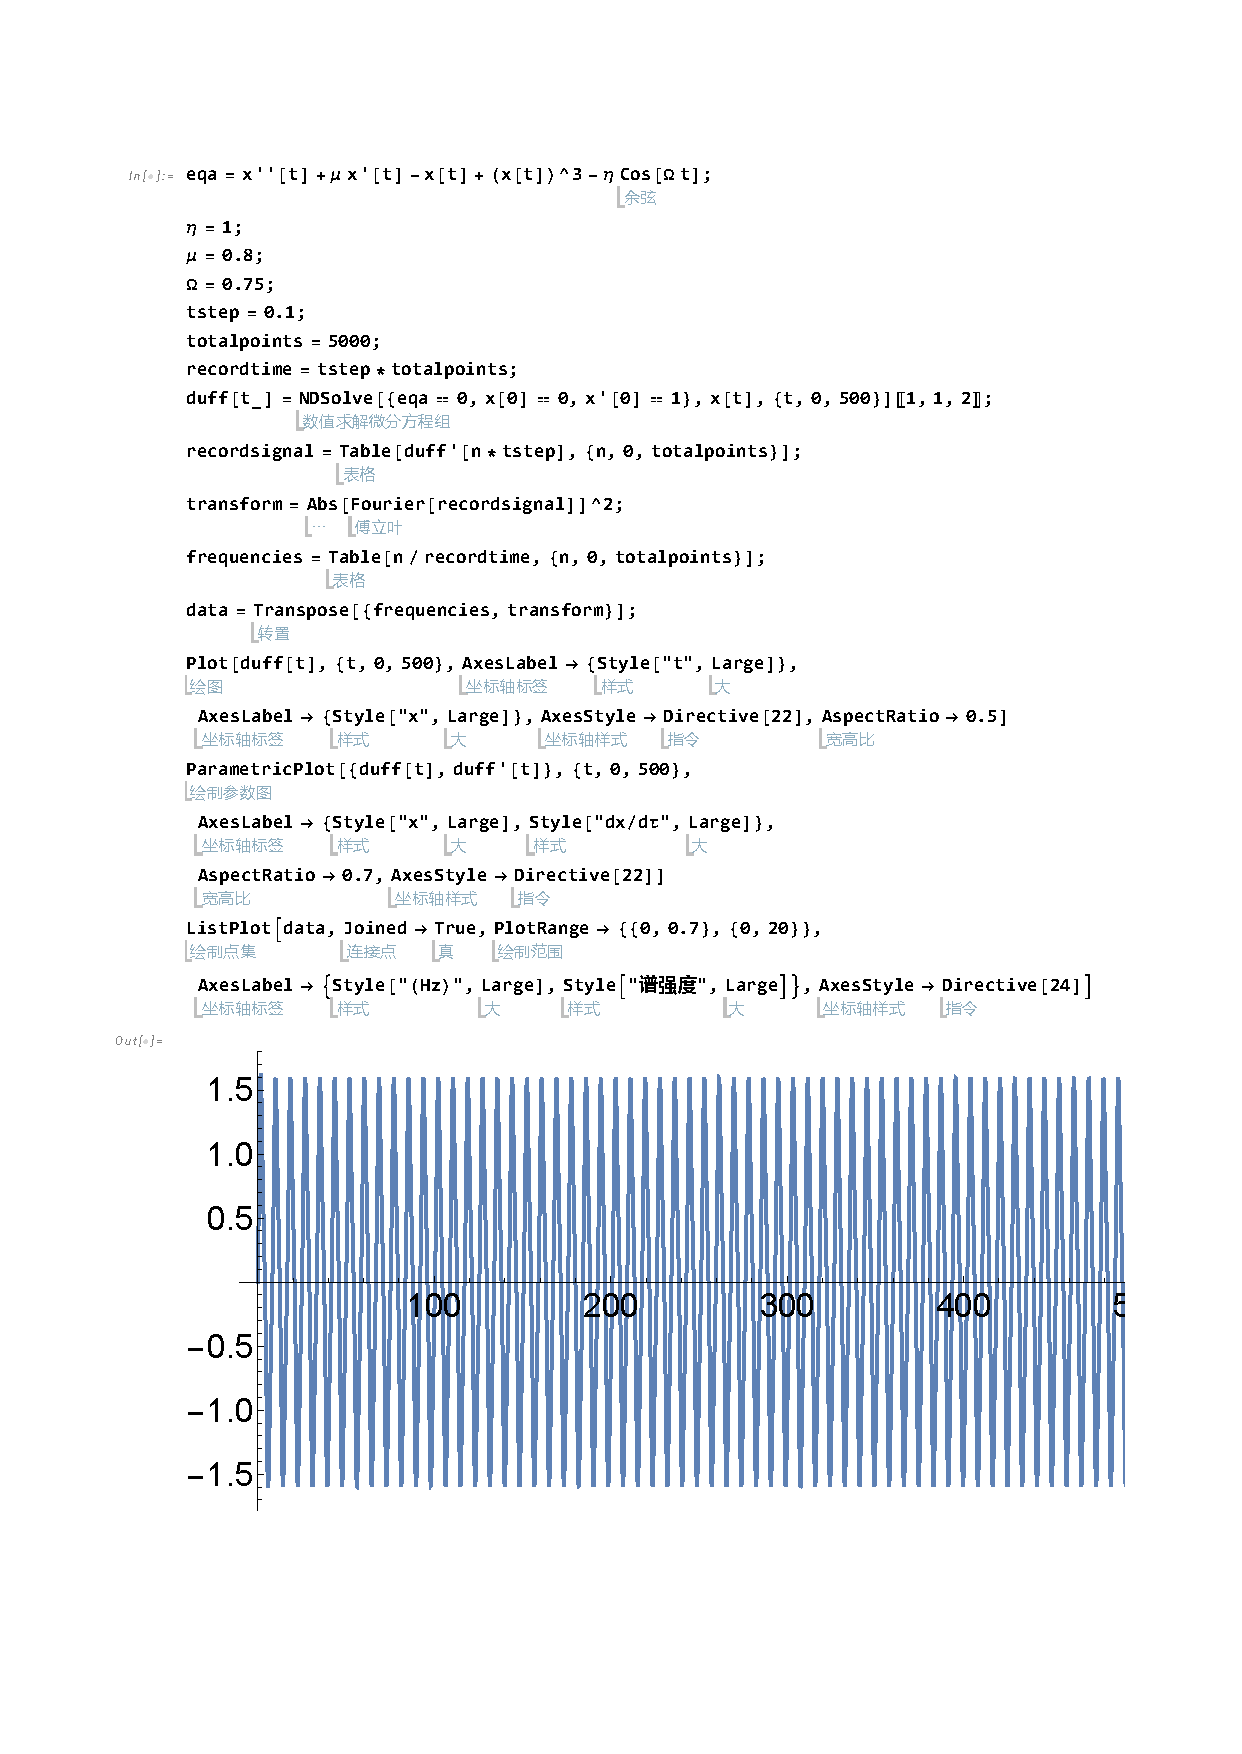
\includepdf[pages=-]{chaos.pdf}
\subsection*{原件扫描}
%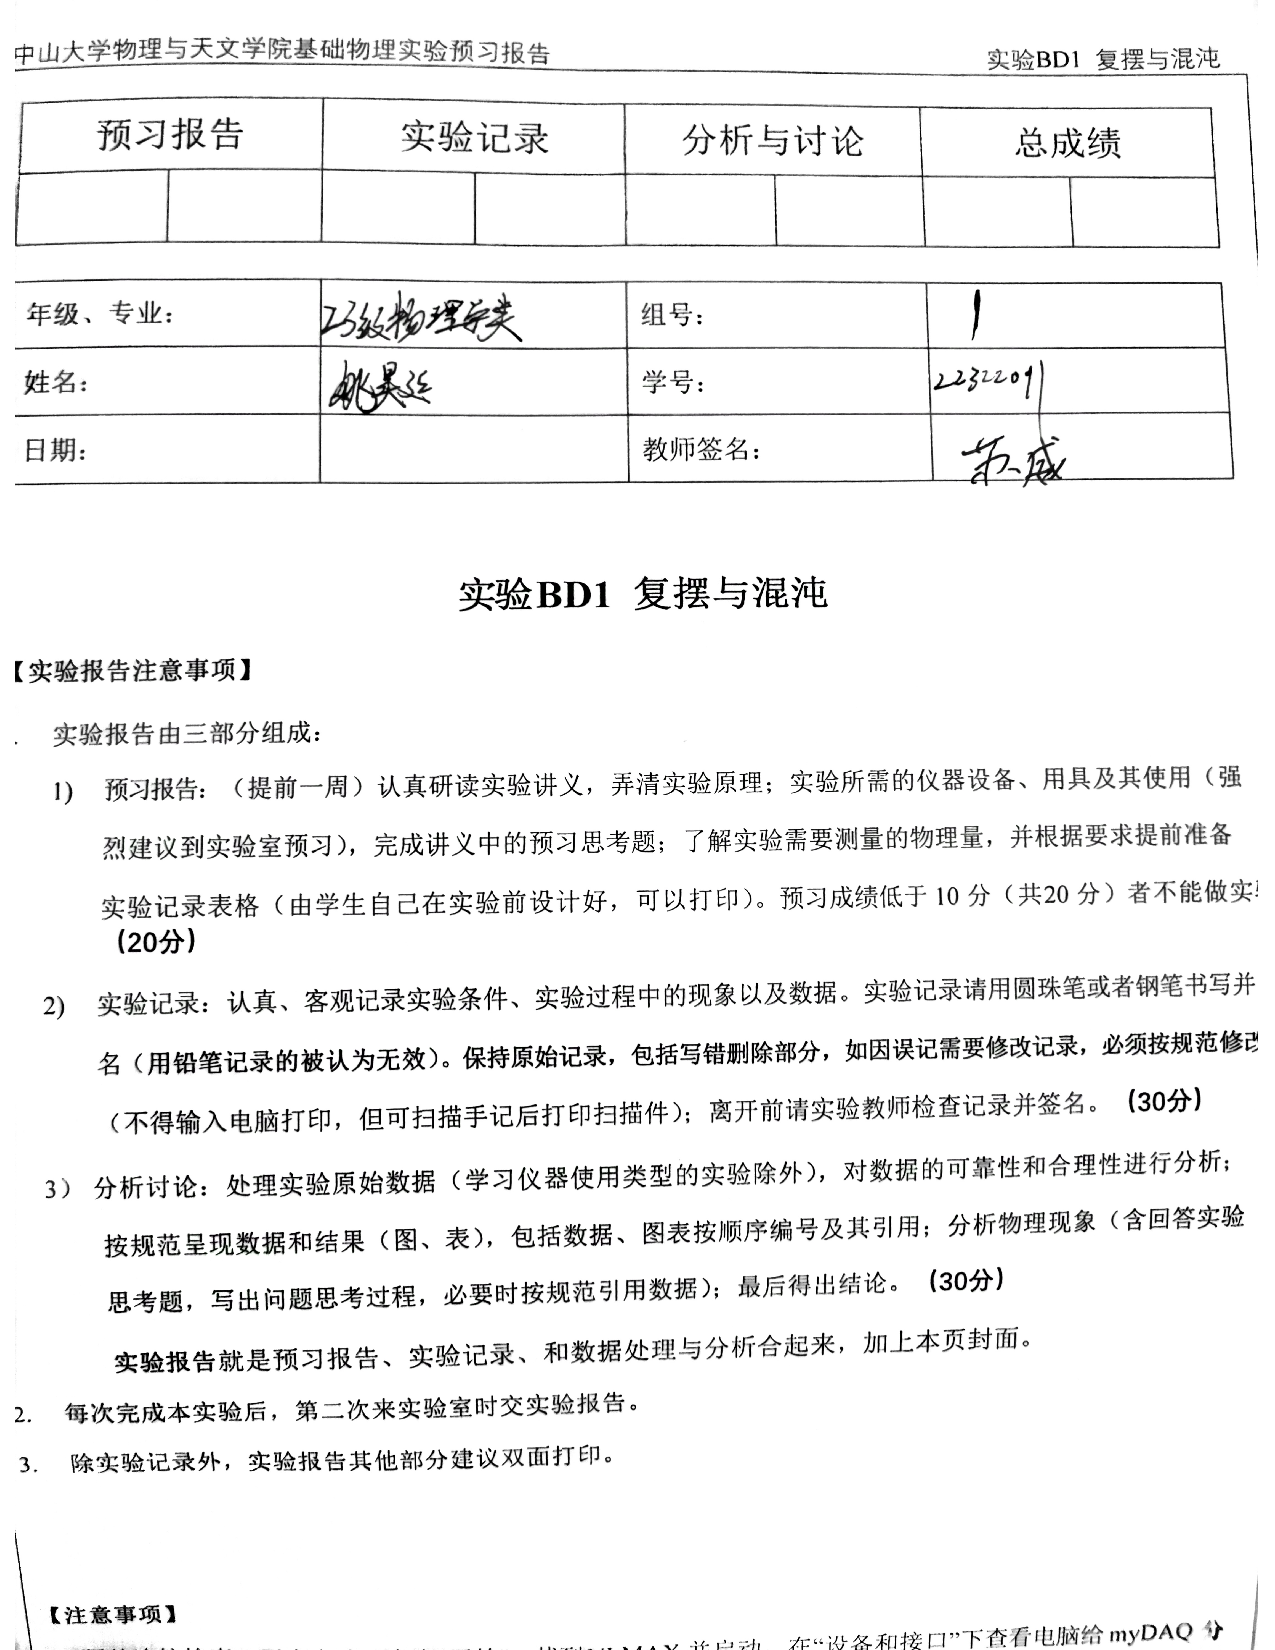
\includepdf[pages=-]{实验3原件.pdf}
\begin{figure}[H]
	\centering
	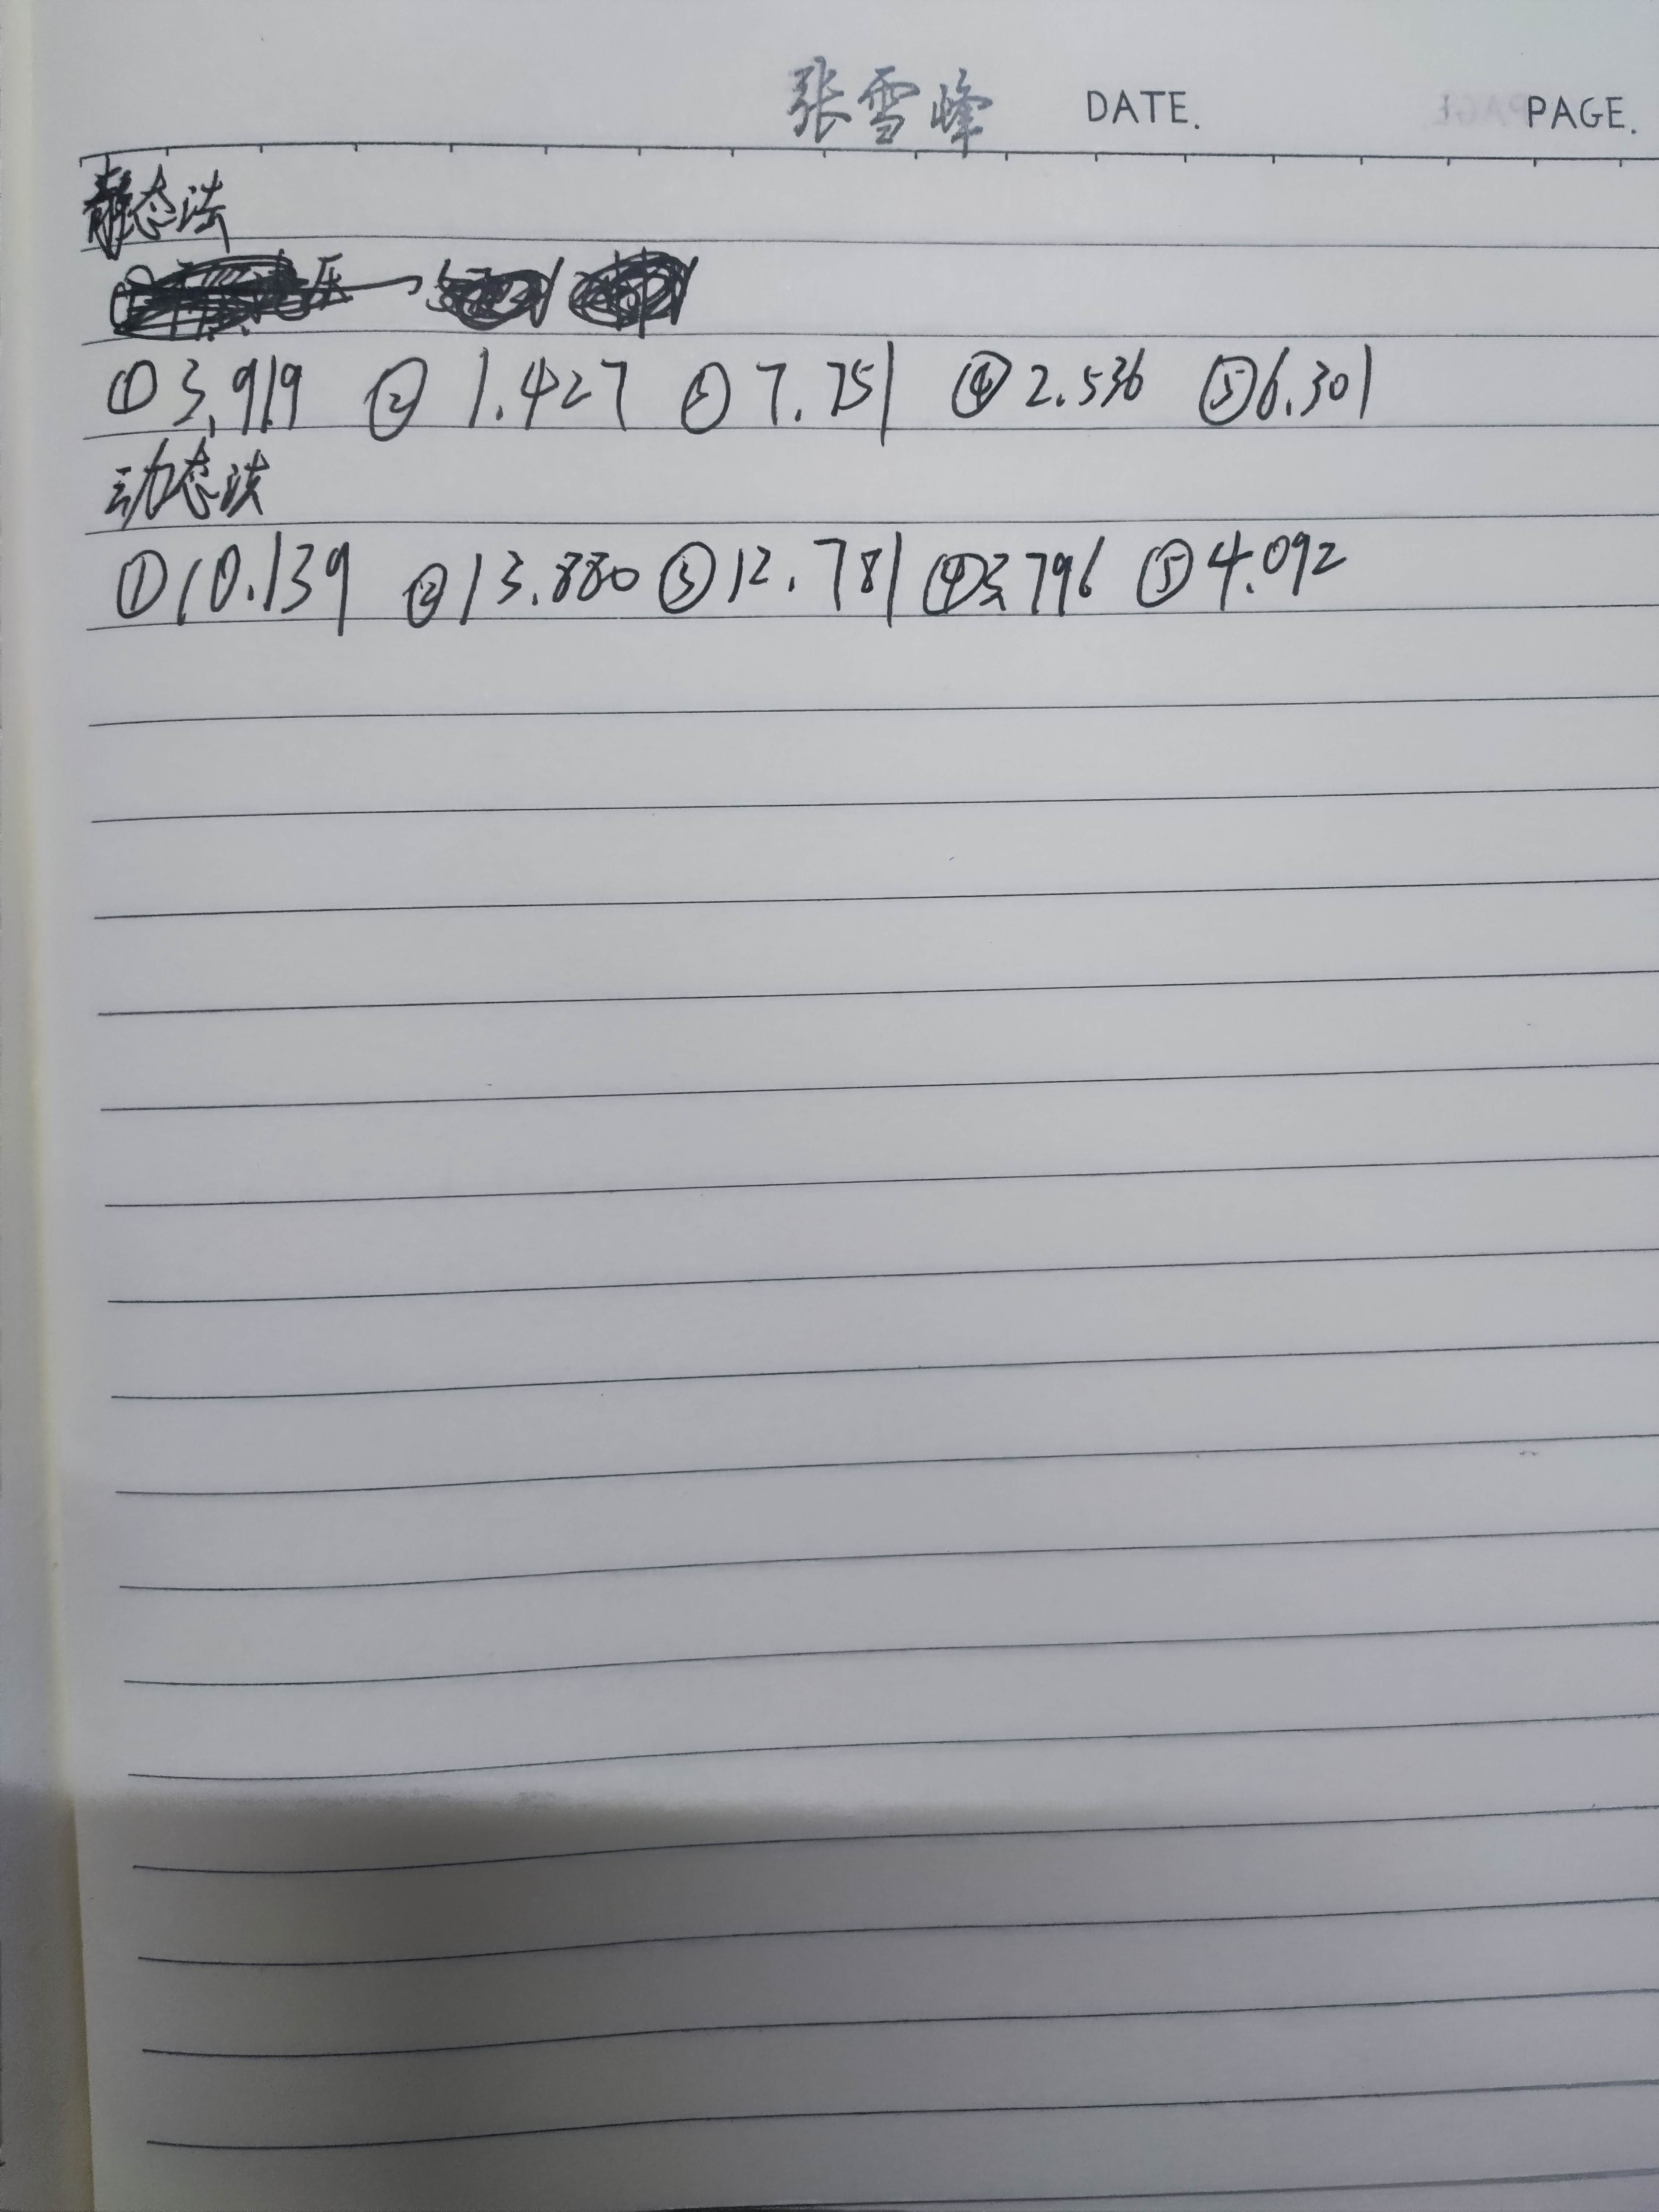
\includegraphics[width=0.4\textwidth]{实验7原件1.jpg}
\end{figure}

\begin{figure}[H]
	\centering
	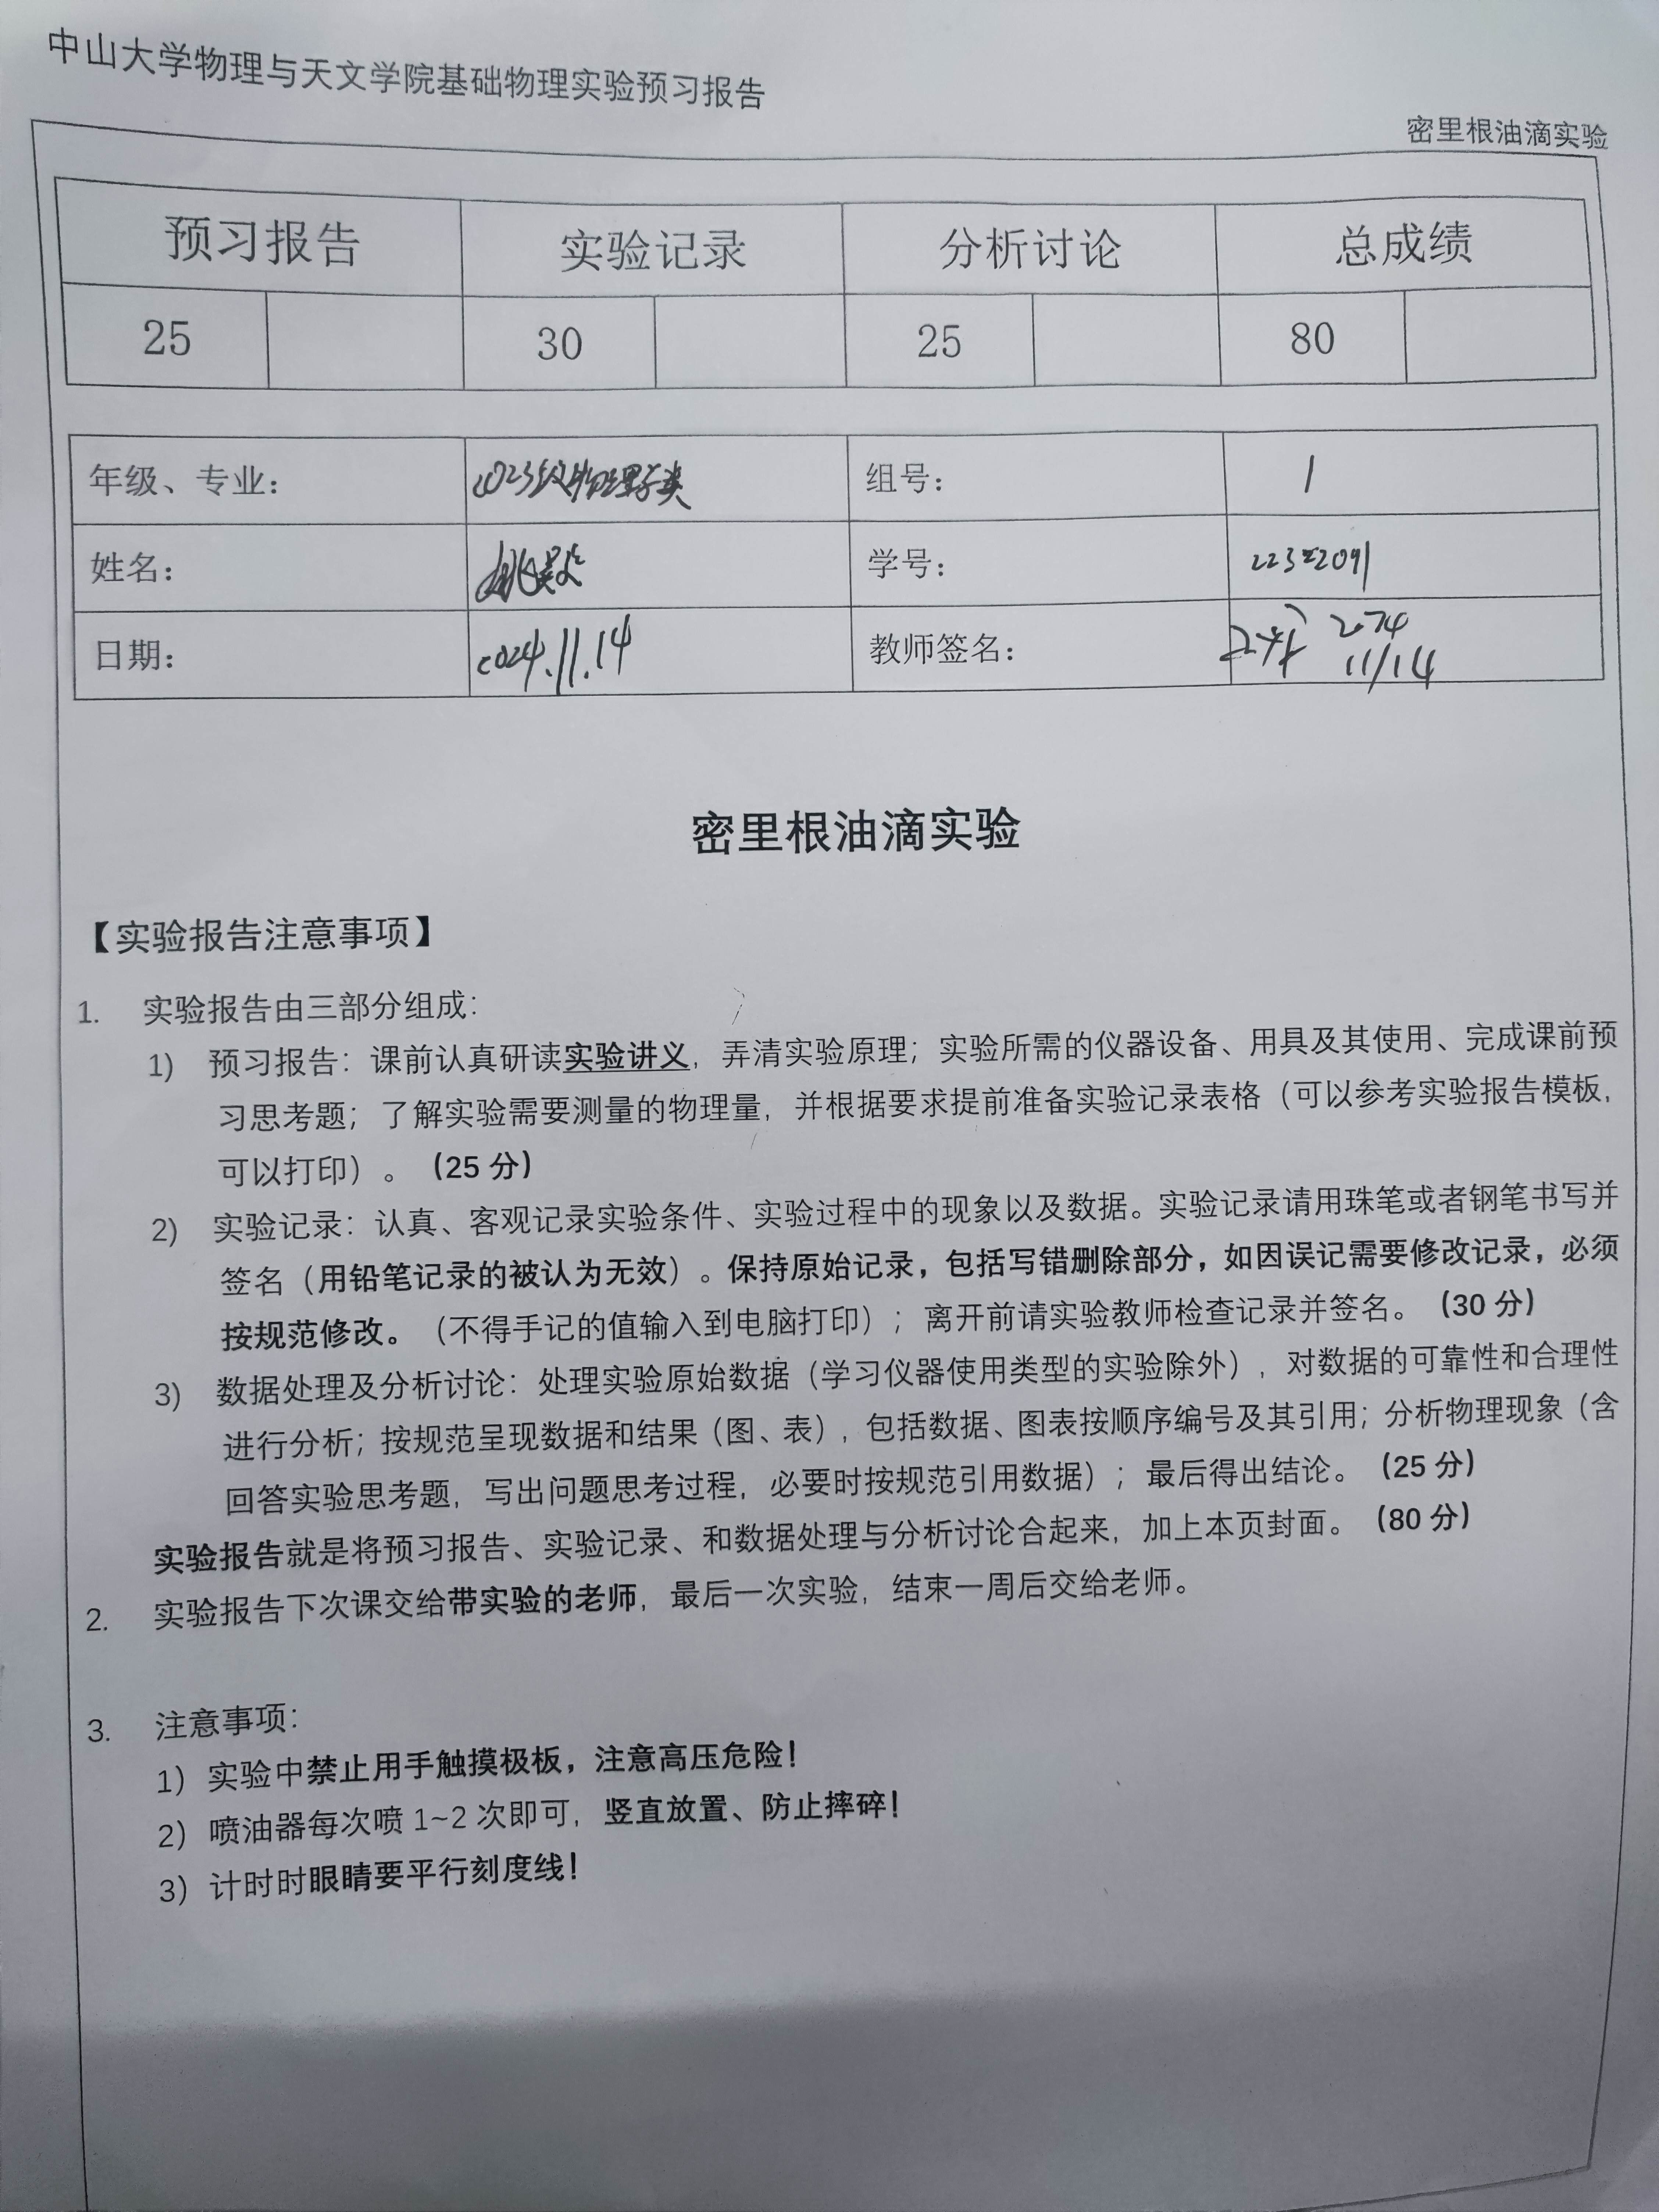
\includegraphics[width=0.4\textwidth]{实验7原件2.jpg}
\end{figure}
\subsection*{桌面}
\begin{figure}[H]
	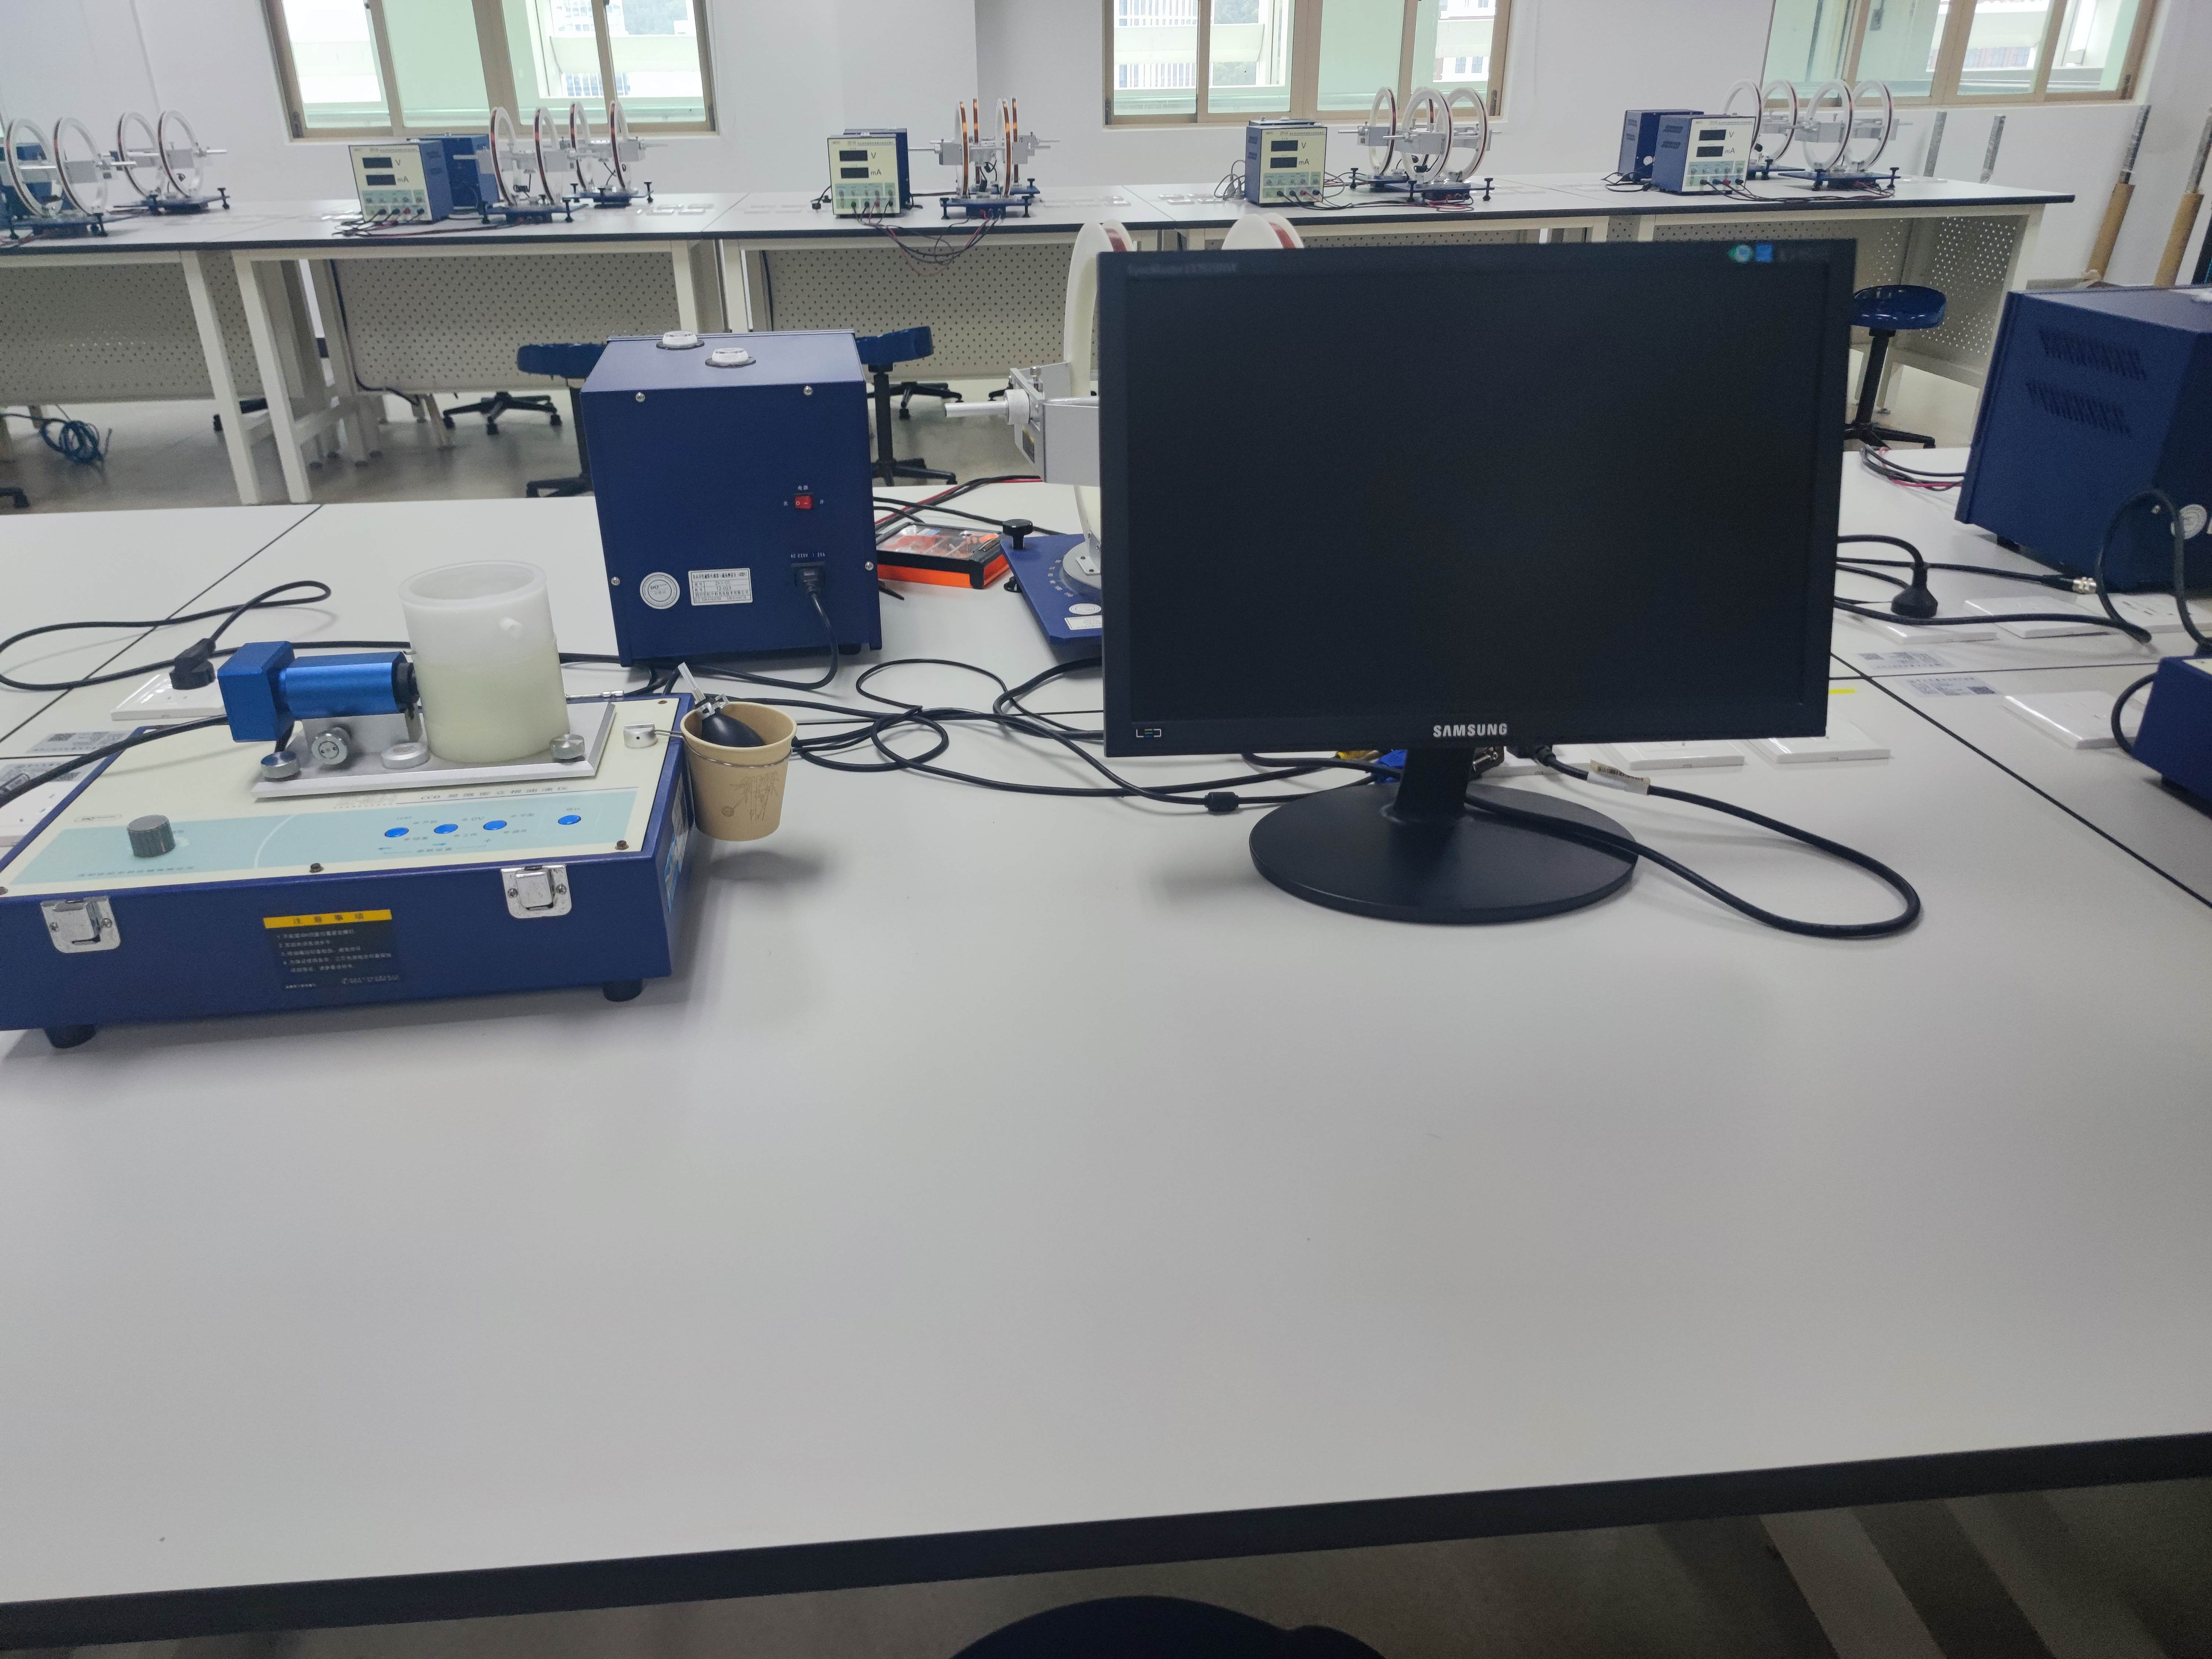
\includegraphics[width=0.95\textwidth]{实验7桌面.jpg}
\end{figure}
\end{document}
